%----------------------------------------------------------------------------------------
%	PACKAGES AND THEMES
%----------------------------------------------------------------------------------------
\documentclass[aspectratio=169,xcolor=dvipsnames]{beamer}

\definecolor{links}{HTML}{2A1B81}
\hypersetup{colorlinks,linkcolor=,urlcolor=links}

\usetheme{Berkeley}

\usepackage{xcolor}
\usepackage{hyperref}
\usepackage{graphicx} % Allows including images
\usepackage{booktabs} % Allows the use of \toprule, \midrule and \bottomrule in tables

%----------------------------------------------------------------------------------------
%	TITLE PAGE
%----------------------------------------------------------------------------------------

% The title
\title[Functional MRI: Part 1 of 2]{Understanding and Interpreting \\Functional Magnetic Resonance Imaging}
\subtitle{Precision Health Boot Camp}

\author[Dr. Alexander Mark Weber] {Alexander Mark Weber}
\institute[UBC] % Your institution may be shorthand to save space
{
    % Your institution for the title page
    Department of Pediatrics, Division of Neurology \\
    University of British Columbia 
    \vskip 3pt
}
\date{12:00 - 2:00 PM \\August 9th, 2022} % Date, can be changed to a custom date


%----------------------------------------------------------------------------------------
%	PRESENTATION SLIDES
%----------------------------------------------------------------------------------------

\begin{document}

\begin{frame}
    % Print the title page as the first slide
    \titlepage
\end{frame}

\begin{frame}{Preamble}

\begin{columns}[c]
\column{0.4\textwidth}
\begin{center}

\includegraphics[width=.7\textwidth]{imgs/Lynne}
\end{center}

\column{0.6\textwidth}


\includegraphics[width=.9\textwidth]{imgs/lit6}

\vspace{.2cm}


\includegraphics[width=.9\textwidth]{imgs/lit7}


\end{columns}
\end{frame}

\begin{frame}{Overview}
    % Throughout your presentation, if you choose to use \section{} and \subsection{} commands, these will automatically be printed on this slide as an overview of your presentation
    \tableofcontents
\end{frame}

%------------------------------------------------
\section{Housekeeping}
%------------------------------------------------

\begin{frame}{Land Acknowledgement}

I would like to acknowledge that we are gathered today on the traditional, ancestral, and unceded territory of the Musqueam people.

\vspace{0.2cm}
\begin{center}
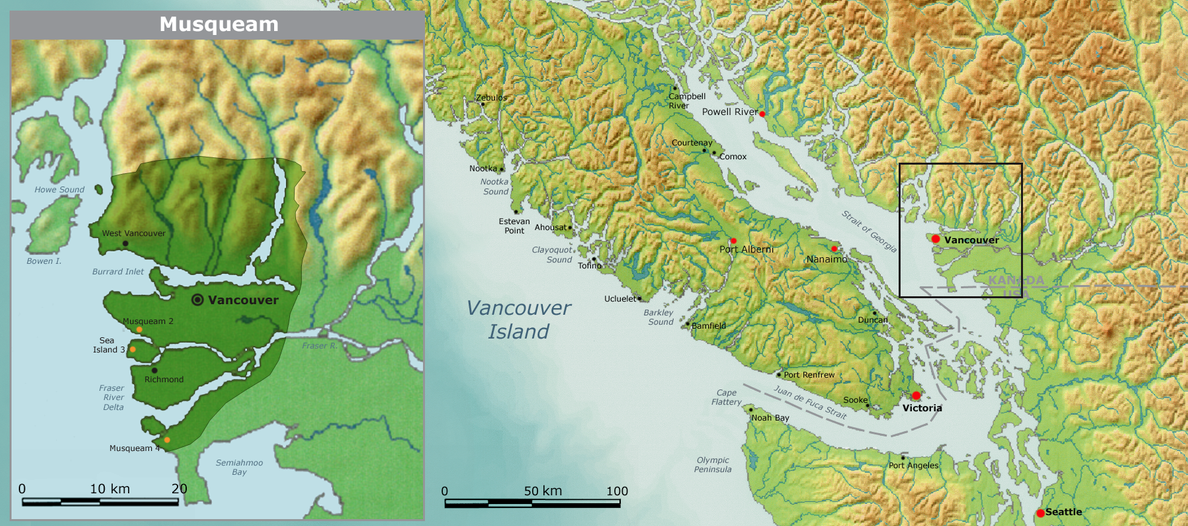
\includegraphics[width=.9\textwidth]{imgs/musqueam}
\end{center}

\end{frame}

%------------------------------------------------

\begin{frame}{Copyright Information}

\begin{columns}[c]
\column{0.5\textwidth}
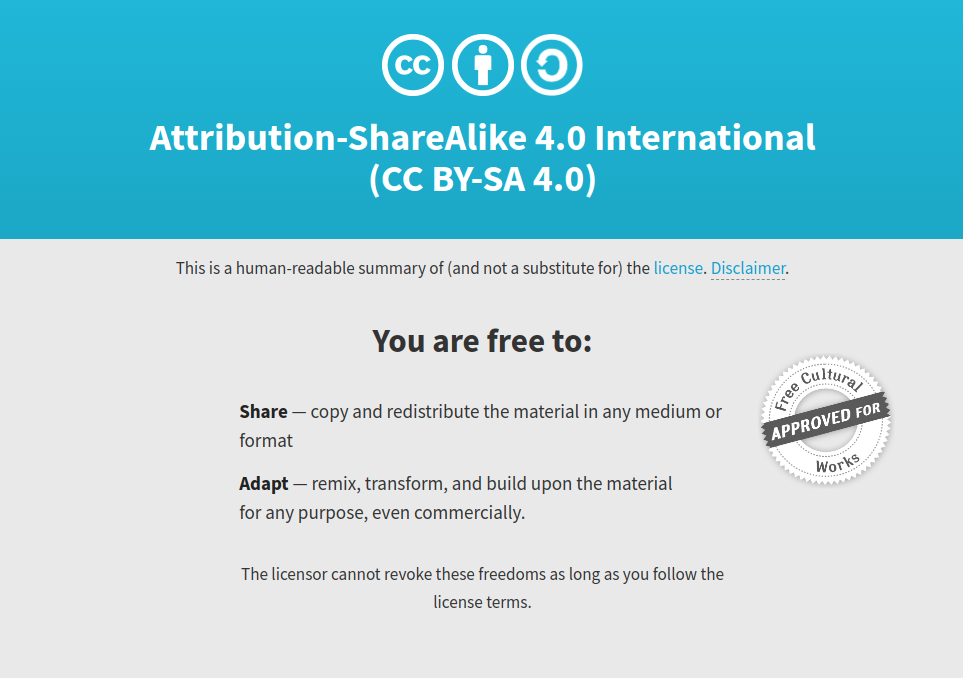
\includegraphics[width=1\textwidth]{imgs/cc}
\column{0.5\textwidth}
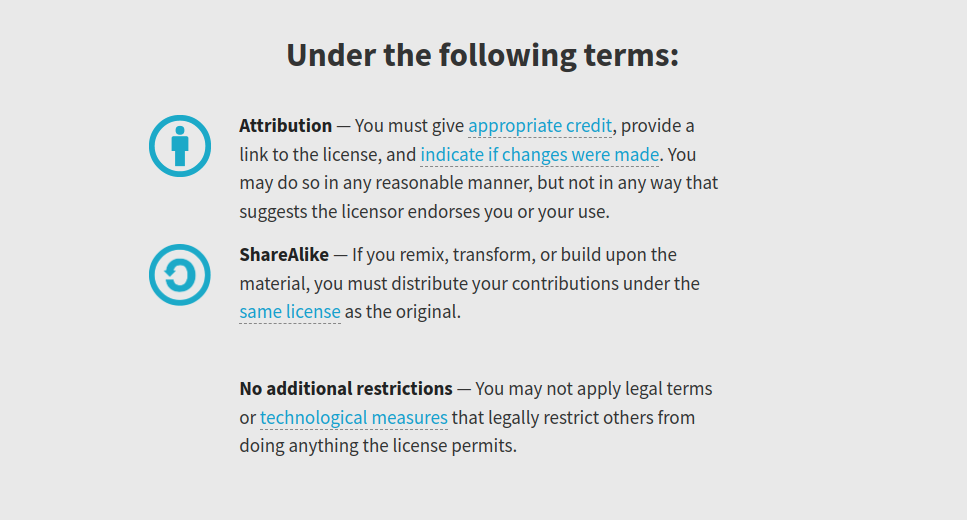
\includegraphics[width=1\textwidth]{imgs/cc2}
\end{columns}

\vspace{.5cm}
Read more here: \url{https://creativecommons.org/licenses/by-sa/4.0/}

\end{frame}

%------------------------------------------------
\section{Freesurfer and DTI Overview}
%------------------------------------------------

\begin{frame}{Freesurfer and DTI Overview}
\begin{columns}[c]
\column<1->{0.45\textwidth}
\vspace{-.4cm}

\begin{center}
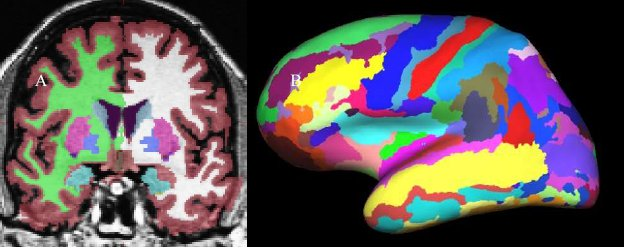
\includegraphics[width=.5\textwidth]{imgs/FSanalysisPipelineFig4}

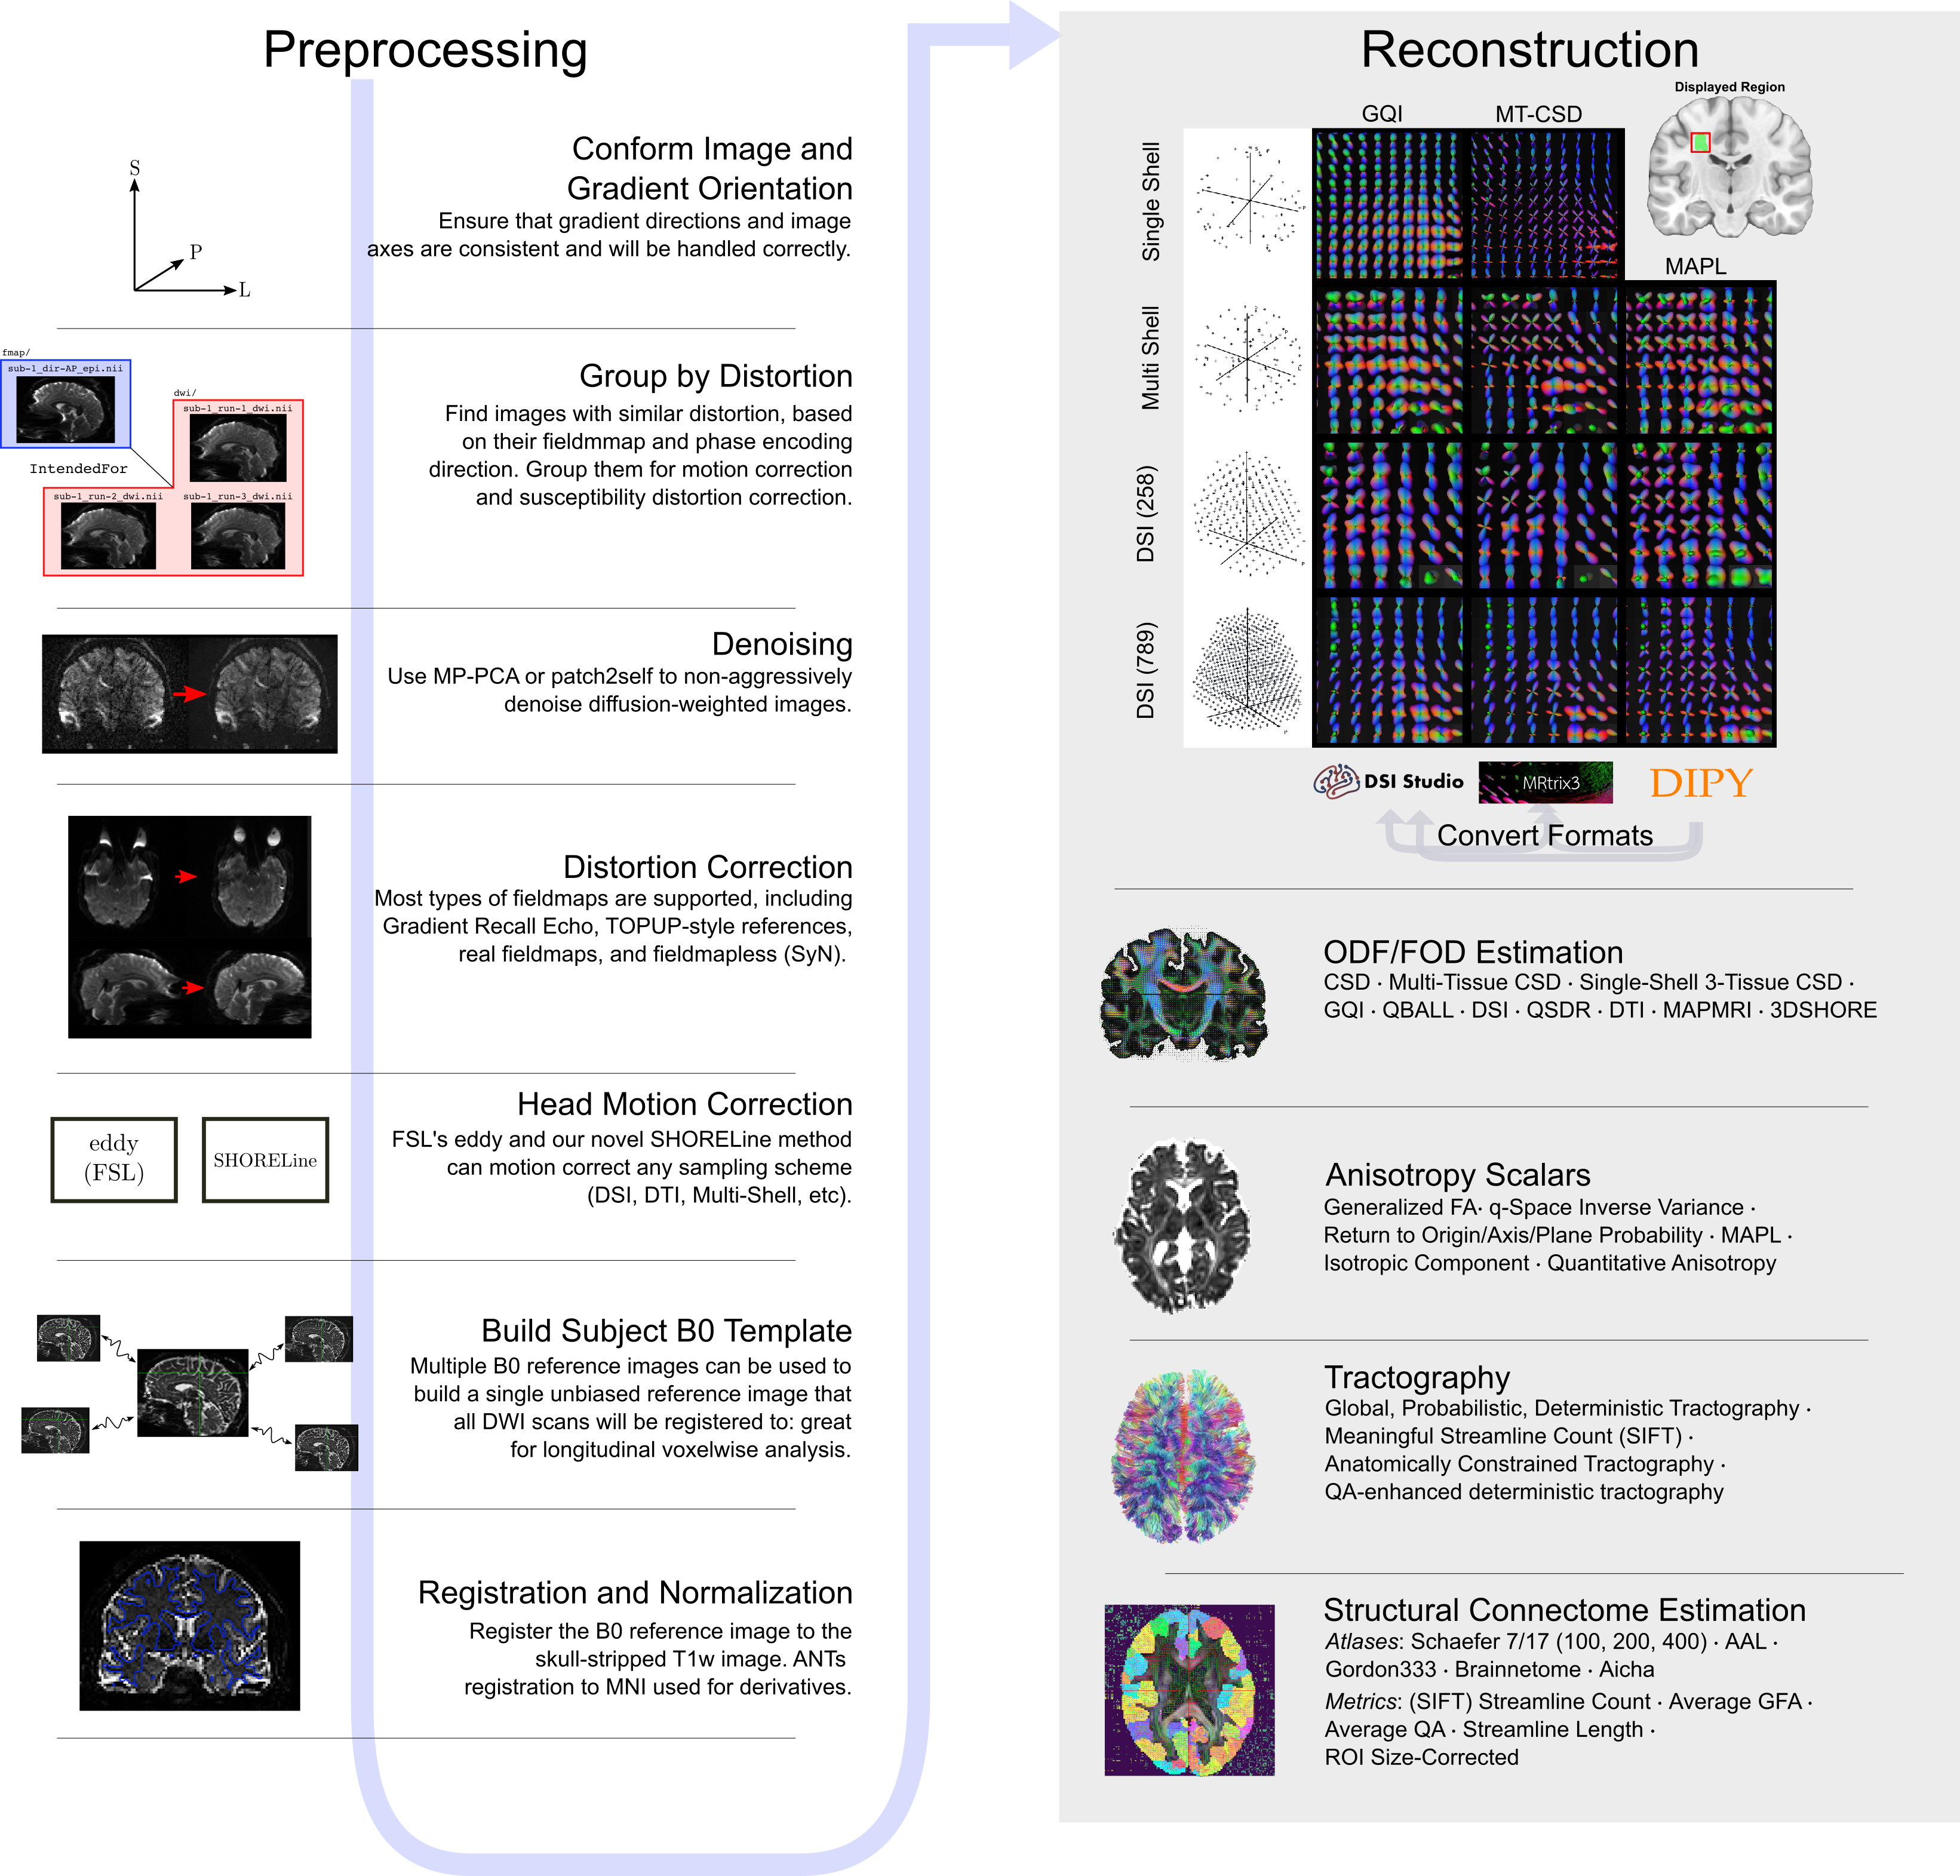
\includegraphics[width=1\textwidth]{imgs/qsiprep_workflow_full}
\tiny{surfer.nmr.mgh.harvard.edu/; }
\end{center}

\column<2->{0.55\textwidth}
Tutorial:
\begin{itemize}
\item Freesurfer
\end{itemize}

Lecture:
\begin{itemize}
\item DTI Physics
\end{itemize}

Tutorial:
\begin{itemize}
\item DTI preprocessing (two ways)
\end{itemize}
\end{columns}

\end{frame}

%------------------------------------------------
\section{Freesurfer Tutorial}
%------------------------------------------------

%------------------------------------------------
\section{MRI Physics: DTI}
%------------------------------------------------






\begin{frame}{Blocks of Highlighted Text}
    In this slide, some important text will be \alert{highlighted} because it's important. Please, don't abuse it.

    \begin{block}{Block}
        Sample text
    \end{block}

    \begin{alertblock}{Alertblock}
        Sample text in red box
    \end{alertblock}

    \begin{examples}
        Sample text in green box. The title of the block is ``Examples".
    \end{examples}
\end{frame}

%------------------------------------------------

\begin{frame}{Multiple Columns}
    \begin{columns}[c] % The "c" option specifies centered vertical alignment while the "t" option is used for top vertical alignment

        \column{.45\textwidth} % Left column and width
        \textbf{Heading}
        \begin{enumerate}
            \item Statement
            \item Explanation
            \item Example
        \end{enumerate}

        \column{.5\textwidth} % Right column and width
        Lorem ipsum dolor sit amet, consectetur adipiscing elit. Integer lectus nisl, ultricies in feugiat rutrum, porttitor sit amet augue. Aliquam ut tortor mauris. Sed volutpat ante purus, quis accumsan dolor.

    \end{columns}
\end{frame}

%------------------------------------------------
\section{Second Section}
%------------------------------------------------

\begin{frame}{Table}
    \begin{table}
        \begin{tabular}{l l l}
            \toprule
            \textbf{Treatments} & \textbf{Response 1} & \textbf{Response 2} \\
            \midrule
            Treatment 1         & 0.0003262           & 0.562               \\
            Treatment 2         & 0.0015681           & 0.910               \\
            Treatment 3         & 0.0009271           & 0.296               \\
            \bottomrule
        \end{tabular}
        \caption{Table caption}
    \end{table}
\end{frame}

%------------------------------------------------

\begin{frame}{Theorem}
    \begin{theorem}[Mass--energy equivalence]
        $E = mc^2$
    \end{theorem}
\end{frame}

%------------------------------------------------

\begin{frame}{Figure}
    Uncomment the code on this slide to include your own image from the same directory as the template .TeX file.
    %\begin{figure}
    %\includegraphics[width=0.8\linewidth]{test}
    %\end{figure}
\end{frame}

%------------------------------------------------

\begin{frame}[fragile] % Need to use the fragile option when verbatim is used in the slide
    \frametitle{Citation}
    An example of the \verb|\cite| command to cite within the presentation:\\~

    This statement requires citation \cite{p1}.
\end{frame}

%------------------------------------------------

\begin{frame}{References}
    % Beamer does not support BibTeX so references must be inserted manually as below
    \footnotesize{
        \begin{thebibliography}{99}
            \bibitem[Smith, 2012]{p1} John Smith (2012)
            \newblock Title of the publication
            \newblock \emph{Journal Name} 12(3), 45 -- 678.
        \end{thebibliography}
    }
\end{frame}

%------------------------------------------------

\begin{frame}
    \Huge{\centerline{The End}}
\end{frame}

%----------------------------------------------------------------------------------------

\end{document}